\documentclass[a4paper]{article} 
\addtolength{\hoffset}{-2.25cm}
\addtolength{\textwidth}{4.5cm}
\addtolength{\voffset}{-3.25cm}
\addtolength{\textheight}{5cm}
\setlength{\parskip}{0pt}
\setlength{\parindent}{0in}

\usepackage[square,sort,comma,numbers]{natbib}
\usepackage{charter} % Use the Charter font
\usepackage[utf8]{inputenc} % Use UTF-8 encoding
\usepackage{microtype} % Slightly tweak font spacing for aesthetics
\usepackage{amsthm, amsmath, amssymb} % Mathematical typesetting
\usepackage{float} % Improved interface for floating objects
\usepackage{hyperref} % For hyperlinks in the PDF
\usepackage{graphicx, multicol} % Enhanced support for graphics
\usepackage{xcolor} % Driver-independent color extensions
%\usepackage{pseudocode} % Environment for specifying algorithms in a natural way
\usepackage[yyyymmdd]{datetime} % Uses YEAR-MONTH-DAY format for dates
\usepackage{subcaption}
\usepackage{fancyhdr} % Headers and footers
\pagestyle{fancy} % All pages have headers and footers
\fancyhead{}\renewcommand{\headrulewidth}{0pt} % Blank out the default header
\fancyfoot[L]{} % Custom footer text
\fancyfoot[C]{} % Custom footer text
\fancyfoot[R]{\thepage} % Custom footer text
\newcommand{\note}[1]{\marginpar{\scriptsize \textcolor{red}{#1}}} % Enables comments in red on margin

%----------------------------------------------------------------------------------------


%-------------------------------
%	TITLE VARIABLES (identify your work!)
%-------------------------------

\newcommand{\yourname}{Mantri Krishna Sri Ipsit} % replace YOURNAME with your name
\newcommand{\yournetid}{180070032} % replace YOURNETID with your NetID
\newcommand{\youremail}{180070032@iitb.ac.in} % replace YOUREMAIL with your email
\newcommand{\assignmentnumber}{1} % replace X with assignment number
\usepackage{verbatim}
\usepackage{xcolor}

\newcommand{\command}[1]{\colorbox{lightgray}{\texttt{#1}}}

\begin{document}

%-------------------------------
%	TITLE SECTION (do not modify unless you really need to)
%-------------------------------
\fancyhead[C]{}
\hrule \medskip
\begin{minipage}{0.295\textwidth} 
\raggedright
\footnotesize
\yourname \hfill\\ 
\yournetid \hfill\\ 
\youremail
\end{minipage}
\begin{minipage}{0.4\textwidth} 
\centering 
\large 
Assignment \assignmentnumber\\ 
\normalsize 
CS 347: Operating Systems\\ 
\end{minipage}
\begin{minipage}{0.295\textwidth} 
\raggedleft
\today\hfill\\
\end{minipage}
\medskip\hrule 
\bigskip


%-------------------------------
%	ASSIGNMENT CONTENT (add your responses)
%-------------------------------

\section*{Part A: Understanding Linux Processes}

\begin{enumerate}
	\item 
	\begin{enumerate}
		\item My machine has \textbf{6} CPU cores. Each core has \textbf{2} threads. Hence the command \command{more /proc/cpuinfo} shows \textbf{12} different processors.
		\item Frequency of each CPU is \textbf{2}.
		\item My system has a total of \textbf{16335724 kB}. Out of this, \textbf{6286200 kB} is free. This is found using the \command{more /proc/meminfo} command.
		\item The total number of forks since bootup is \textbf{24541}. And the total number of context switches since bootup is \textbf{87459116}. This is found using the \command{more /proc/stat} command.
	\end{enumerate}
	\item 
	\begin{enumerate}
		\item The PID of the process running the \texttt{cpu} command is \textbf{24831}.
		\item This process is consuming \textbf{100\%} of CPU and \textbf{0\%} of memory.
		\item The current state of the process is \textbf{R}. It is in \textbf{running} state.
	\end{enumerate}
	\item 
	\begin{enumerate}
		\item The PID of the process spawned by the shell to run the \texttt{cpu-print} executable is \textbf{27038}. This is found using the \command{ps -C cpu-print} command.
		\item The PID of the parent of the \texttt{cpu-print} process is \textbf{11168}. This is found using the \command{ps -f -C cpu-print} command. The PIDs of all ancestors found using \command{pstree -sp 11168} are:
		\verbatiminput{ancestors.txt}
		\item Using the \command{ls -l /proc/32077/fd} (here 32077 is the PID of the output redirection process) command, we get the following:
		\verbatiminput{fd.txt}
		Here we can see that the file descriptor for standard output is being pointed to \texttt{/tmp/tmp.txt} while the other descriptors are pointing towards a pseudo-terminal. Hence we can say that the I/O redirection happens in the following way: \textbf{\textit{First, based on the redirection type ($<$, $>$, or $2>$), a file is opened (if it already exists then that will be used) with the given filename and then in the process, the file descriptor will point to the new file opened. In that way, whenever a system call is made to print to a screen or throw an error or take input, the data is sent to the file to which the file descriptor points to.}}
	\end{enumerate}
	\item 
		\begin{enumerate}
			\item In the program, there is a loop that runs 4 times. Inside each loop, \texttt{fork()} is called. Hence the processes created can be explained using the following flow chart:
			\begin{figure}[ht]
				\centering
				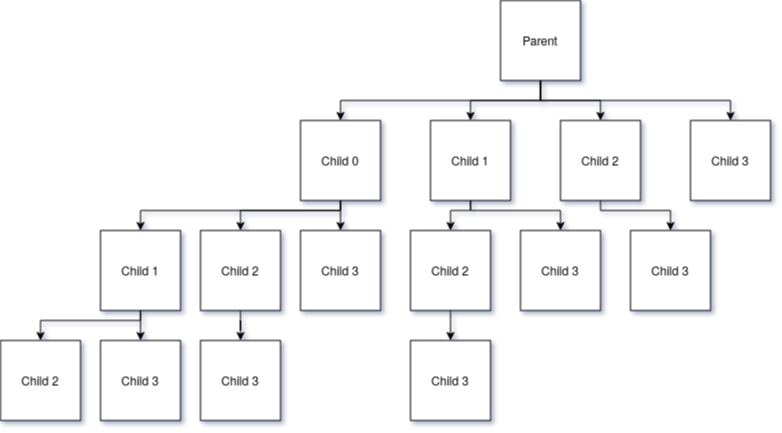
\includegraphics[scale=0.4]{flowchart.png}
			\end{figure}
		
			As we can see here, the output of \texttt{fork4.c} program should contain \textbf{1} line of child 0, \textbf{2} lines of child 1, \textbf{4} lines of child 2 and \textbf{8} lines of child 3. The order in which these lines are printed is based on the scheduling algorithm the OS is using. But theoritically, whenever a \texttt{fork()} is called, the parent and the created child execute concurrently. 
			\item The program has been modified as follows:
			 \verbatiminput{../fork4_wait.c}
			 This is nothing but the parent waits for the child to finish its process. So as expected, rge children will be reaped in a depth-first order, i.e., the most recently created child will be reaped first. Here is the output of the modified program above:
			 \verbatiminput{./fork4_wait_output.txt}
		\end{enumerate}
\end{enumerate}

\section*{Part B: A Simple Shell}

\end{document}
